\providecommand{\main}{../main}
\documentclass[\main/main.tex]{subfiles}
\graphicspath{{../images/}}
\begin{document}
\section{
    相関関数
}
\subsection{
    相関関数への制限
}
共形変換対称性が相関関数に与える制限を求める。
作用と経路積分測度が共形変換に対して不変であるとき、
\begin{align}
    \⟨𝒪₁(x₁)⋯𝒪_N(x_N)\⟩
    = \⟨𝒪'₁(x'₁)⋯𝒪'_N(x'_N)\⟩
\end{align}
が成り立つ。
これは全空間で積分したWard-Takahashi恒等式
\begin{align}
    \⟨Q_a\Q\Big(𝒪₁(x₁)⋯𝒪_N(x_N))\⟩
    = ∑_{n=1}^N \⟨𝒪₁(x₁)⋯𝒬_a𝒪ₙ(x)⋯𝒪_N(x_N)\⟩ = 0
\end{align}
から導くこともできる。
これは以下のように図示される。
\begin{figure}[H]
    \centering
    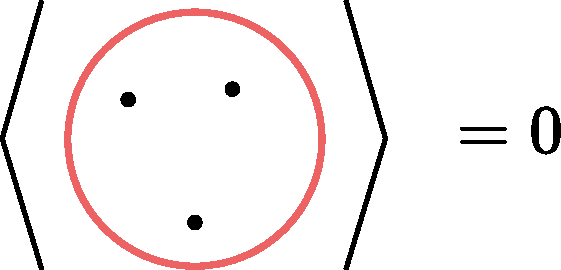
\includegraphics[width=0.25\hsize]{../images/conformal symmetry of correlation function.pdf}
    \caption{トポロジカル演算子が全ての演算子を囲む場合、期待値はゼロになる。}
\end{figure}

ここで$𝒪ₙ$をスカラープライマリー場とし、
\begin{align}
    g_{μν}(x) → g'_{μν}(x') = Ω(x)^2g_{μν}(x)
\end{align}
に対して、
\begin{align}
    𝒪'ₙ(x'ₙ) = Ω(xₙ)^{Δₙ}𝒪ₙ(xₙ)
\end{align}
となるとする。このとき、
\begin{align}
    \⟨𝒪₁(x₁)⋯𝒪ₙ(xₙ)\⟩
    =Ω(x_1)^{-Δ_1}⋯Ω(x_N)^{-Δ_N}\⟨𝒪₁(x'₁)⋯𝒪_N(x'_N)\⟩
    \label{correlation of primaries}
\end{align}
となる。
\subsection{
    2点関数
}
まずスカラープライマリー場の2点関数を考える。
並進対称性、回転対称性から
\begin{align}
    \⟨𝒪₁(x₁)𝒪₂(x₂)\⟩
    &
    = \⟨𝒪₁(x₁-x₂)𝒪₂(0)\⟩
    \∅ &
    = \⟨𝒪₁(|x₁-x₂|e)𝒪₂(0)\⟩
\end{align}
と書ける。ただし、$e=(1,0,0,…)$とした。
つまり相関関数は$|x₁-x₂|$のみに依存する。
さらに$𝒪₁,𝒪₂$の共形次元をそれぞれ$Δ₁,Δ₂$とおくと、(\ref{correlation of primaries})から定数$C₁₂$によって
\begin{align}
    \⟨𝒪₁(x₁)𝒪₂(x₂)\⟩ = \f{C₁₂}{|x₁-x₂|^{Δ₁+Δ₂}}
\end{align}
と書ける。これで相関関数の座標依存性が決定されてしまった。

さらに特殊共形変換を考えてみる。
\begin{align}
    x^μ → x'^μ = \f{x^μ+x²c^μ}{1+2c⋅x+c²x²}
\end{align}
に対し、計量は
\begin{align}
    g'_{μν} = Ω(x)^2g_{μν},\␣
    Ω(x) = 1-2c⋅x+c²x²
\end{align}
となる。これは特殊共形変換を反転と並進の合成として
\begin{align}
    x^μ → \f{x^μ}{x²} → \f{x^μ}{x²} - c^μ
    → \f{x^μ/x²-c^μ}{(x/x²-c)²}
\end{align}
と表した時、2回の反転によってスケールが$1/x²(x/x²-c)²$倍されることによる。
したがって、
\begin{align}
    \⟨𝒪₁(x₁)𝒪₂(x₂)\⟩
    = \f{1}{Ω₁^{Δ₁}Ω₂^{Δ₂}}\⟨𝒪₁(x₁')𝒪₂(x₂')\⟩
    \label{CWTI: correlation restriction by SCT}
\end{align}
となる。ここで$Ωⱼ = 1-2c⋅xⱼ + c²xⱼ²$と定義した。
さらに、反転変換について
\begin{align}
    \Q(\f{x_1}{x_1^2}-\f{x_2}{x_2^2})^2
    = \f{(x_1-x_2)^2}{x_1^2x_2^2}
\end{align}
が成り立つことから
\begin{align}
    (x'₁-x₂')²
    = \f{
        (x_1/x_1^2-x_2/x_2^2)^2
    }{
        (x_1/x_1^2-c)^2(x_2/x_2^2-c)^2
    }
    = \f{(x_1-x_2)^2}{Ω_1Ω_2}
\end{align}
となるので、
(\ref{CWTI: correlation restriction by SCT})
は
\begin{align}
    \f{C₁₂}{|x₁-x₂|^{Δ₁+Δ₂}}
    = \f{(Ω₁Ω₂)^{(Δ₁+Δ₂)/2}}{Ω₁^{Δ₁}Ω₂^{Δ₂}}
        \f{C₁₂}{|x₁-x₂|^{Δ₁+Δ₂}}
\end{align}
となる。これが成り立つのは$Δ₁=Δ₂$のときのみである。
したがって、
\begin{align}\tcboxmath{
    \⟨𝒪₁(x₁)𝒪₂(x₂)\⟩ = \f{C₁₂δ_{Δ₁Δ₂}}{|x₁-x₂|^{2Δ₁}}
}\end{align}
となる。
すなわち共形不変性の帰結として、共形次元が異なる場の相関関数は$0$である。

\subsection{
    3点関数
}
次に3点関数$\⟨𝒪₁(x₁)𝒪₂(x₂)𝒪₃(x₃)\⟩$を考える。
並進対称性と回転対称性から相関関数は$xᵢⱼ=|xᵢ-xⱼ|$の関数となる。
またスケール不変性から、
\begin{align}
    \⟨𝒪₁(x₁)𝒪₂(x₂)𝒪₃(x₃)\⟩
    &
    = ∑_{a,b,c} \f{C_{123}^{abc}}
        {x_{12}^a x_{23}^b x_{31}^c}
\end{align}
と書ける。ただし、$a,b,c$は$a+b+c = Δ₁+Δ₂+Δ₃$満たすとする。
次に特殊共形変換を考えると、
\begin{align}
    \f{C_{123}^{abc}}{x_{12}^a x_{23}^b x_{31}^c}
    = \f{
        (Ω₁Ω₂)^{a/2}(Ω₂Ω₃)^{b/2}(Ω₃Ω₁)^{c/2}
    }{
        Ω₁^{Δ₁}Ω₂^{Δ₂}Ω₃^{Δ₃}
    }\f{
        C_{123}^{abc}
    }{
        x_{12}^a x_{23}^b x_{31}^c
    }
\end{align}
となる。
ここから、
\begin{align}
    a+b = 2Δ₂,\␣
    b+c = 2Δ₃,\␣
    c+a = 2Δ₁
\end{align}
が分かる。
これを解いて、
\begin{align}
    a = Δ₁+Δ₂-Δ₃,\␣
    b = Δ₂+Δ₃-Δ₁,\␣
    c = Δ₃+Δ₁-Δ₂
\end{align}
となるので、3点関数は定数$f_{123}$によって
\begin{align}\tcboxmath{
    \⟨𝒪₁(x₁)𝒪₂(x₂)𝒪₃(x₃)\⟩
    = \f{f₁₂₃}{x_{12}^{Δ₁+Δ₂-Δ₃}x_{23}^{Δ₂+Δ₃-Δ₁}x_{31}^{Δ₃+Δ₁-Δ₂}}
}\end{align}
と書ける。

\subsection{
    4点関数
}
次に4点関数$\⟨𝒪₁(x₁)𝒪₂(x₂)𝒪₃(x₃)𝒪₄(x₄)\⟩$を考える。
並進対称性と回転対称性から相関関数は$xᵢⱼ=|xᵢ-xⱼ|$の関数となる。
またスケール不変性から、
\begin{align}
    \⟨𝒪₁(x₁)𝒪₂(x₂)𝒪₃(x₃)𝒪₄(x₄)\⟩
    &
    = ∑_{a,b,c,d,e,f}
    \f{
        C_{1234}^{abcdeef}
    }{
        x_{12}^a x_{13}^b x_{14}^c
        x_{23}^d x_{24}^e x_{34}^f
    }
    \label{four point function under scale inv.}
\end{align}
と書ける。ただし、$a+b+c+d+e+f = Δ₁+Δ₂+Δ₃+Δ₄$が成り立つとする。
しかし3点関数の場合と異なり特殊共形変換に対する変換性から$a,b,c,d,e,f$を求めることはできない。
実際、複比(crossratio)
\begin{align}
    u = \f{x_{12}²x_{34}²}{x_{13}²x_{24}²},\␣
    v = \f{x_{14}²x_{23}²}{x_{13}²x_{24}²}
    \label{def of crossratio}
\end{align}
が共形変換で不変な量となっており、$u,v$のどのようなべきも許されるからである。$u,v$は明らかに並進・回転・スケール変換について不変であり、特殊共形変換についても
\begin{align}
    u → \f{(Ω₁Ω₃)(Ω₂Ω₄)}{(Ω₁Ω₂)(Ω₃Ω₄)}u = u,\␣
    v → \f{(Ω₁Ω₃)(Ω₂Ω₄)}{(Ω₁Ω₄)(Ω₂Ω₃)}v = v
\end{align}
から不変であることが分かる。
また、他に共形変換で保たれる量がないことは、以下のようにして分かる。
\begin{itemize}
    \item 特殊共形変換によって$x₄$を無限遠点に移す。
    \item 並進によって$x₁$を原点に移す。
    \item 回転とスケール変換によって$x₃$を$(1,0,0,…)$に移す。
    \item $x₃$を不変に保つ回転によって$x₂$を$(x,y,0,0,…)$に移す。
\end{itemize}
すると、自由度は2つのパラメーター$x,y$のみである。
したがって、共形不変な独立なパラメーターが2つだけであることが分かる。
$z = x+\i y$とおくと、$u,v$は
\begin{align}
    u = x_{12}² = z\=z,\␣
    v = x_{23}² = (1-z)(1-\=z)
    \label{relation between crossratio and z}
\end{align}
と書ける。

(\ref{four point function under scale inv.})において、$u,v$のべきを括り出してまとめると、
\begin{align}
    \⟨𝒪₁(x₁)⋯𝒪₄(x₄)\⟩
    = ∑_{a,b,c,e}
    \f{
        C_{1234}^{abce}(u,v)
    }{
        x_{12}^a x_{13}^b x_{14}^c x_{24}^e
    }
\end{align}
と書ける。特殊共形変換に対する変換性から、
\begin{align}
    a+b+c = 2Δ₁,\␣
    a+e = 2Δ₂,\␣
    b = 2Δ₃,\␣
    c+e = 2Δ₄
\end{align}
となるので、これを解いて
\begin{align}
    a = Δ₁+Δ₂-Δ₃-Δ₄,\␣
    b = 2Δ₃,\␣
    c = Δ₁-Δ₂-Δ₃+Δ₄,\␣
    d = -Δ₁+Δ₂+Δ₃+Δ₄
\end{align}
を得る。したがって、
\begin{align}
    \⟨𝒪₁(x₁)⋯𝒪₄(x₄)\⟩
    = \f{C(u,v)}{x_{12}^{Δ₁+Δ₂-Δ₃-Δ₄}x_{13}^{2Δ₃}x_{14}^{Δ₁-Δ₂-Δ₃+Δ₄}x_{24}^{-Δ₁+Δ₂+Δ₃+Δ₄}}
\end{align}
と書ける。さらに慣例に従って、以下のように書き直す。
\begin{align}\tcboxmath{
    \⟨𝒪₁(x₁)⋯𝒪₄(x₄)\⟩
    = \f{
        g(u,v)
    }{
        x_{12}^{Δ₁+Δ₂}x_{34}^{Δ₃+Δ₄}
    }
    \Q(\f{x_{24}}{x_{14}})^{Δ₁-Δ₂}
    \Q(\f{x_{14}}{x_{13}})^{Δ₃-Δ₄}
    \label{four point function}
}\end{align}
$g(u,v) = u^{Δ₃+Δ₄}C(u,v)$は任意の関数である。
特に同一のスカラープライマリー場の4点関数は
\begin{align}
    \⟨ϕ(x₁)⋯ϕ(x₄)\⟩
    = \f{g(u,v)}{x_{12}^{2Δ_ϕ}x_{34}^{2Δ_ϕ}}
\end{align}
と書ける。
% 共形不変性からはこれ以上のことは言えないが、後で演算子積展開との無撞着性から$g(u,v)$を制限できることを見る。

\subsection{
    テンソル演算子の相関関数
}
テンソルプライマリー演算子の相関関数も、共形不変性によって制限を受ける。
ここでは結果だけを述べることにする。
1階のテンソルプライマリー演算子の2点関数は、
\begin{gather}
    \⟨𝒪^μ(x)𝒪_ν(y)\⟩
    = C_𝒪 \f{{I^μ}_ν(x-y)}{|x-y|^{2Δ}},
    \\
    {I^μ}_ν(x) = δ^μ_ν - 2\f{x^μx_ν}{x^2}
\end{gather}
と計算される。
% これが共形不変性を満たすことは、反転変換
% \begin{align}
%     \~x = \f{x}{x^2},\␣
%     \∂{x^μ}{\~x^ν} = x^2{I^μ}_ν(x)
% \end{align}
% に対する以下の関係式を示れば十分である。
% \begin{align}
%     \⟨J_μ(\~x)J_ν(\~y)\⟩
%     = x^{2Δ}y^{2Δ}{I_μ}^ρ(x){I_ν}^σ(y)\⟨J_ρ(x)J_σ(y)\⟩
% \end{align}
% これは少し計算すれば示すことができる。
% \begin{align}
%     \f{1}{|\~x-\~y|^{2Δ}}
%     = \f{x^{2Δ}y^{2Δ}}{|x-y|^{2Δ}}
% \end{align}
% \begin{align}
%     I_{μν}(\~x-\~y)
%     &
%     = δ_{μν}
%     - 2\f{(\~x_μ-\~y_μ)(\~x_ν-\~y_ν)}{(\~x-\~y)^2}
%     \∅ &
%     = δ_{μν}
%     -2\f{x^2y^2(\~x_μ-\~y_μ)(\~x_ν-\~y_ν)}{(x-y)^2}
% \end{align}
% \begin{align}
%     &
%     \f{x^2y^2(\~x_μ-\~y_μ)(\~x_ν-\~y_ν)}{(x-y)^2}
%     \∅ &
%     = \f{y^2}{(x-y)^2}\f{x_μx_ν}{x^2}
%     +\f{x^2}{(x-y)^2}\f{y_μy_ν}{y^2}
%     -\f{x_μy_ν+y_μx_ν}{(x-y)^2}
%     \∅ &
%     =\f{y^2-x^2}{(x-y)^2}\f{x_μx_ν}{x^2}
%     +\f{x^2-y^2}{(x-y)^2}\f{y_μy_ν}{y^2}
%     +\f{(x_μ-y_μ)(x_ν-y_ν)}{(x-y)^2}
%     \∅ &
%     =\Q(1-2\f{x⋅(x-y)}{(x-y)^2})\f{x_μx_ν}{x^2}
%     +\Q(1+2\f{y⋅(x-y)}{(x-y)^2})\f{y_μy_ν}{y^2}
%     +\f{(x_μ-y_μ)(x_ν-y_ν)}{(x-y)^2}
% \end{align}
% \begin{align}
%     &
%     {I_μ}^ρ(x){I_ν}^σ(y)I_{ρσ}(x-y)
%     \∅ &
%     = \Q(δ^ρ_μ-2\f{x_μx^ρ}{x^2})
%     \Q(δ^σ_ν-2\f{y_νy^σ}{y^2})
%     \Q(δ_{ρσ}-2\f{(x_ρ-y_ρ)(x_σ-y_σ)}{(x-y)^2})
%     \∅ &
%     = δ_{μν}
%     -2\f{(x_μ-y_μ)(x_ν-y_ν)}{(x-y)^2}
%     \∅ &
%     -2\f{x_μx^ρ}{x^2}\Q(δ_{ρν}-2\f{(x_ρ-y_ρ)(x_ν-y_ν)}{(x-y)^2})
%     -2\f{y_νy^σ}{y^2}\Q(δ_{μσ}-2\f{(x_μ-y_μ)(x_σ-y_σ)}{(x-y)^2})
%     \∅ &\␣
%     + 4\f{x_μy_νx^ρy^σ}{x^2y^2}
%         \Q(δ_{ρσ}-2\f{(x_ρ-y_ρ)(x_σ-y_σ)}{(x-y)^2})
% \end{align}
% \begin{align}
%     &
%     \f{x⋅(x-y)x_μ(x_ν-y_ν)}{x^2(x-y)^2}
%     +\f{y⋅(x-y)(x_μ-y_μ)y_ν}{y^2(x-y)^2}
%     \∅ &
%     +\f{(x⋅y)x_μy_ν}{x^2y^2}
%     -\f{2x⋅(x-y)y⋅(x-y)x_μy_ν}{x^2y^2(x-y)^2}
%     \∅ &
%     = \f{x⋅(x-y)x_μx_ν}{x^2(x-y)^2}
%     -\f{y⋅(x-y)y_μy_ν}{y^(x-y)^2}
% \end{align}
またスピン$l$
\footnote{
    $l$階の対称トレースレステンソルのこと
}のテンソルに対しては、
\begin{align}
    \⟨𝒪^{μ_1⋯μ_l}(x)𝒪_{ν_1⋯ν_l}(0)\⟩
    =C_𝒪\l(
        \f{
            {I^{μ_1}}_{ν_1}(x)⋯{I^{μ_l}}_{ν_l}(x)
        }{
            x^{2Δ}
        }
        +\t{perms}-\t{traces}
    \r)
\end{align}
となる。
permsは$μ$の添字を入れ替えた項を表しており、tracesは$δ^{μ_iμ_j},δ_{ν_iν_j}$に比例するようなトレース部分を表す。
次に3点関数については
\begin{gather}
    \⟨ϕ₁(x₁)ϕ₂(x₂)𝒪^{μ₁⋯μₗ}(x₃)\⟩
    = \f{
        f_{ϕ₁ϕ₂𝒪}(Z^{μ_1}⋯Z^{μ_l}-\t{traces})
    }{
        x_{12}^{Δ₁+Δ₂-Δ₃+l}
        x_{23}^{Δ₂+Δ₃-Δ₁-l}
        x_{31}^{Δ₃+Δ₁-Δ₂-l},
    }
    \\
    Z^μ ≔ \f{x_{13}^μ}{x_{13}^2}-\f{x_{23}^μ}{x_{23}^2}
\end{gather}
となる。
これらを導出するために空間埋め込み法を用いるのが便利である。
詳しくは、\cite{Nakayama_2019}の10章や\cite{Costa_2011}
を参照してほしい。

% \subsection{
%     空間埋め込み法
% }

% \printbibliography
\end{document}